\title{Lecture 17\\Representation of Temporal Entities in a Knowledge Base}

\begin{frame}
	\titlepage
\end{frame}

\begin{frame}{\\Lecture outline}
	\topline
	\justifying
	Temporal entities and their classification. Describing how events are related. Causal relationships and their representation in a knowledge base. Processes, situations, and events. Temporal relations and their representation in a knowledge base.
\end{frame}

\begin{frame}{\\Temporal entities}
	\topline
	\justifying
	\scnheader{temporal entity}
	\scnidtf{time-varying entity}
	\scnidtf{non-stationary entity}
	\scnidtf{entity that has a beginning, an end, or both}
	\scnidtf{entity with temporal characteristics (such as duration, a starting instant, and an ending instant)}
	\begin{scnrelfromset}{partition}
		\scnitem{past entity}
		\scnitem{current entity}
		\scnitem{future entity}
	\end{scnrelfromset}
\end{frame}

\begin{frame}{\\Temporal entities}
	\topline
	\justifying
	\scnheader{temporal entity}
	\begin{scnrelfromset}{partition}
		\scnitem{time-dependent connection}
		\scnitem{temporal structure}
		\begin{scnindent}
			\scnidtf{structure containing at least one temporal entity}
		\end{scnindent}
		\scnitem{material entity}
	\end{scnrelfromset}
\end{frame}

\begin{frame}{\\Classification of temporal entities}
	\topline
	\justifying
	\setlength{\emergencystretch}{2em}
	\scnheader{temporal entity}
	\begin{scnrelfromset}{partition}
		\scnitem{continuous temporal entity}
			\begin{scnindent}
			\begin{scnrelfromset}{partition}
				\scnitem{point-like temporal entity}
						\begin{scnindent}
						\scnidtf{atomic (instantaneous) temporal entity}
						\end{scnindent}
				\scnitem{extended continuous temporal entity}
			\end{scnrelfromset}
			\end{scnindent}
		\scnitem{discrete temporal entity}
				\begin{scnindent}
				\scnidtf{temporal entity that can be decomposed into a sequence of point-like temporal entities}
				\end{scnindent}
		\scnitem{intermittent temporal entity}
			\begin{scnindent}
			\scnidtf{temporal entity with interruptions}
			\end{scnindent}
	\end{scnrelfromset}
\end{frame}

\begin{frame}{\\Time-dependent connections}
	\topline
	\justifying
	Every time-dependent connection is a tuple belonging to the set of temporal entities.\\
	A temporal connection, by contrast, is itself a permanent
	entity that describes how temporal entities are related in time.
\end{frame}

\begin{frame}{\\Processes, situations, and events}
	\topline
	\justifying
	\scnheader{temporal structure}
	\begin{scnrelfromset}{partition}
		\scnitem{situation}
		\begin{scnindent}
			\scnidtf{static temporal structure}
		\end{scnindent}
		\scnitem{process}
		\begin{scnindent}
			\scnidtf{dynamic temporal structure}
		\end{scnindent}
	\end{scnrelfromset}
\end{frame}

\begin{frame}{\\Situation}
	\topline
	\justifying
	A situation is a structure with at least one temporal entity as an element. If it contains several temporal entities, there is a moment in the past, present, or future when they all exist simultaneously.

	\scnheader{situation}
	\scnidtf{state of a dynamic system described at a given level of detail}
\end{frame}

\begin{frame}{\\Process}
	\topline
	\justifying

	\vspace{10mm}
	A process is defined by the appearance or disappearance of connections between a given temporal entity and other entities.\\
	A process can be associated with its \textbf{\textit{initial situation*}} and \textbf{\textit{final situation*}}, the situations between which the transition takes place during the process.
	\scnheader{process}
	\scnidtf{dynamic structure}
	\scnidtf{process that transforms a temporal entity from one state into another}

\end{frame}

\begin{frame}{\\Event}
	\topline
	\justifying
	\scnheader{event}
	\scnidtf{boundary point of a temporal entity}
	\scnidtf{point-like temporal entity marking the start, the completion, or both of another temporal entity
	(for example, a process)}
\end{frame}

\begin{frame}{\\Event}
	\topline
	\justifying
	\vspace{10mm}
	\begin{SCn}
		\begin{figure}[H]
			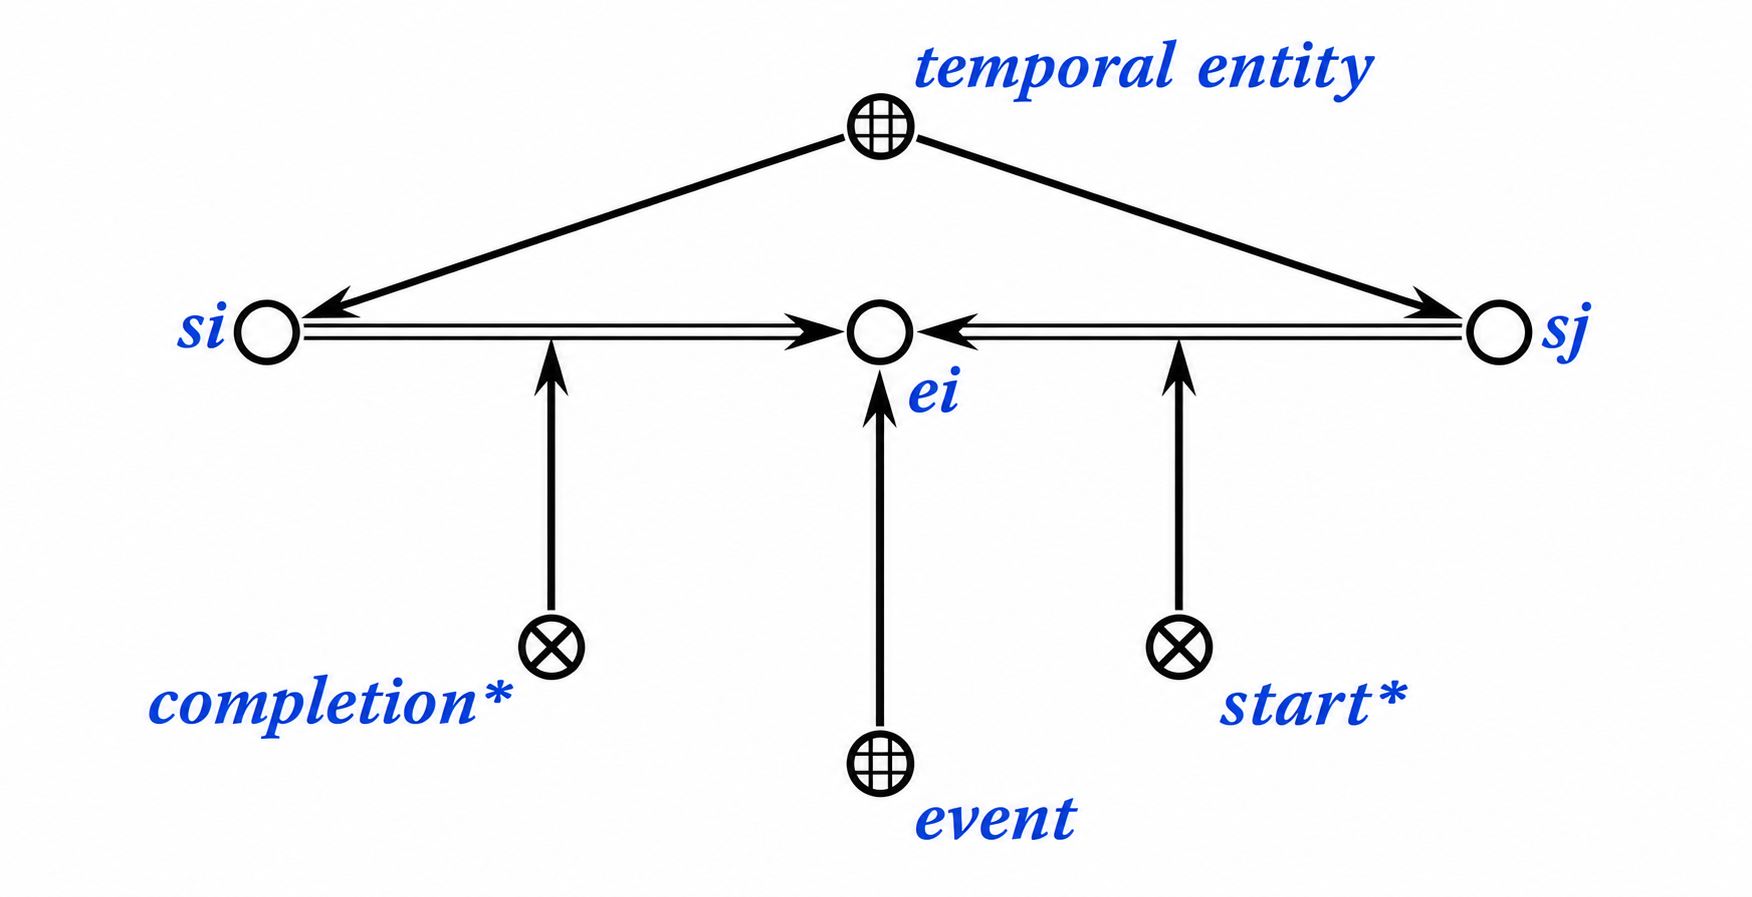
\includegraphics[width=\linewidth,height=0.68\textheight,keepaspectratio]{figures/sd_temp_entities/event_en.png}
		\end{figure}
	\end{SCn}
\end{frame}

\begin{frame}{\\\textbf{\textit{event*}}}
	\topline
	\justifying
	\scnheader{event*}
	\scniselement{binary relation}
	\scntext{explanation}{Tuples of the \textit{event*} relation connect the sign of a process to an ordered pair. Its first component is the sign of the process's \textit{initial situation*}, and its second is the sign of its \textit{final situation*}}
\end{frame}

\begin{frame}{\\\textbf{\textit{event*}}}
	\topline
	\justifying
	\vspace{10mm}
	\begin{SCn}
		\begin{figure}[H]
			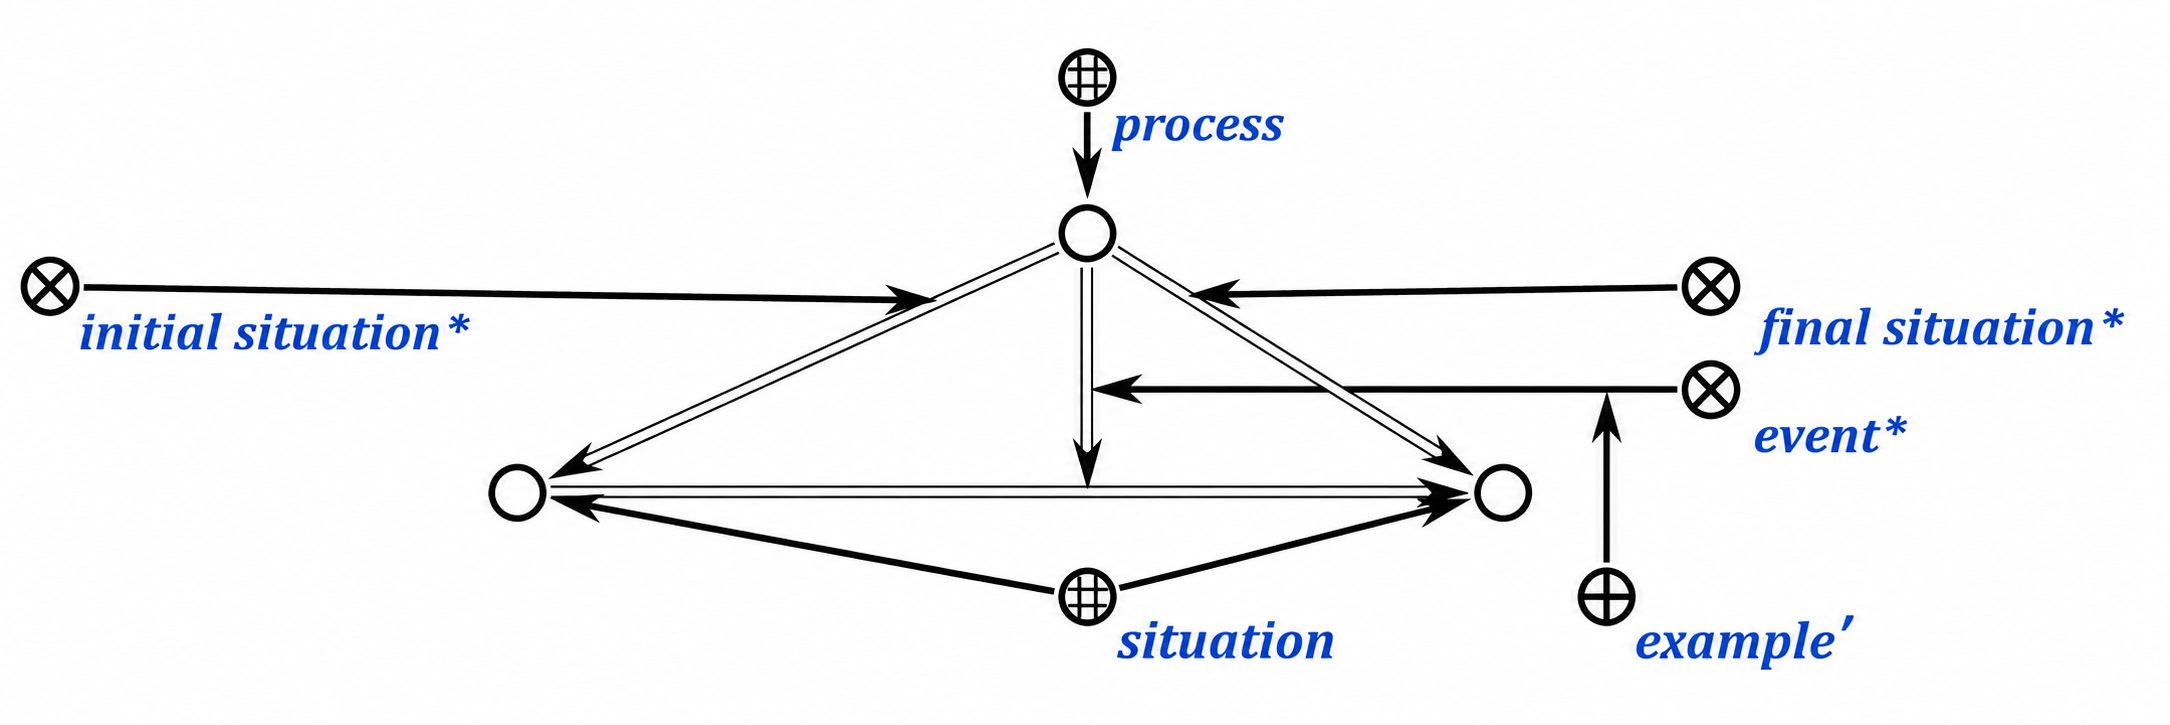
\includegraphics[width=\linewidth,height=0.68\textheight,keepaspectratio]{figures/sd_temp_entities/nrel_event_en.png}
		\end{figure}
	\end{SCn}
\end{frame}

\begin{frame}{\\Example of a situation}
	\topline
	\justifying
	\vspace{10mm}
	\begin{SCn}
		\begin{figure}[H]
			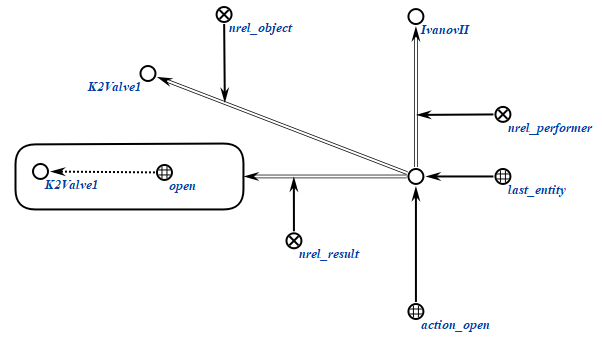
\includegraphics[width=\linewidth,height=0.68\textheight,keepaspectratio]{figures/sd_temp_entities/valve_opening.png}
		\end{figure}
	\end{SCn}
\end{frame}

\begin{frame}{\\Example of a process}
\topline
\justifying
\vspace{10mm}
\begin{SCn}
	\begin{figure}[H]
		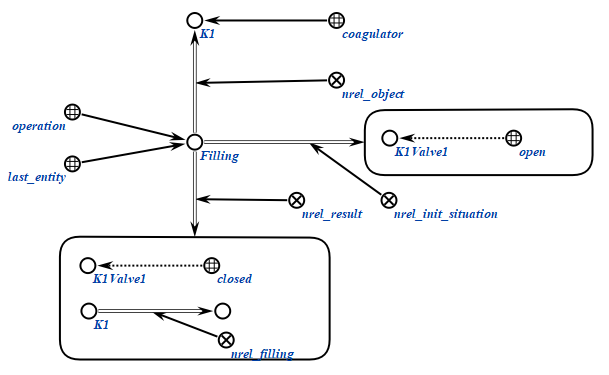
\includegraphics[width=\linewidth,height=0.68\textheight,keepaspectratio]{figures/sd_temp_entities/process_description.png}
	\end{figure}
\end{SCn}
\end{frame}

\begin{frame}{Temporal relations}
	\topline
	\justifying
	\scnheader{temporal relation}
	\scnrelto{family of subsets}{temporal connection}
	\scnhaselement{temporal inclusion*}
	\scnhaselement{temporal union*}
	\scnhaselement{temporal decomposition*}
	\scnhaselement{temporal sequence*}
	\begin{scnindent}
		\begin{scnrelfromset}{partition}
			\scnitem{temporal adjacency*}
			\scnitem{temporal sequence with a gap*}
			\scnitem{temporal sequence with overlap*}
		\end{scnrelfromset}
	\end{scnindent}
\end{frame}

\begin{frame}{\\Temporal decomposition}
	\topline
	\justifying
	\vspace{10mm}
	\begin{SCn}
		\begin{figure}[H]
			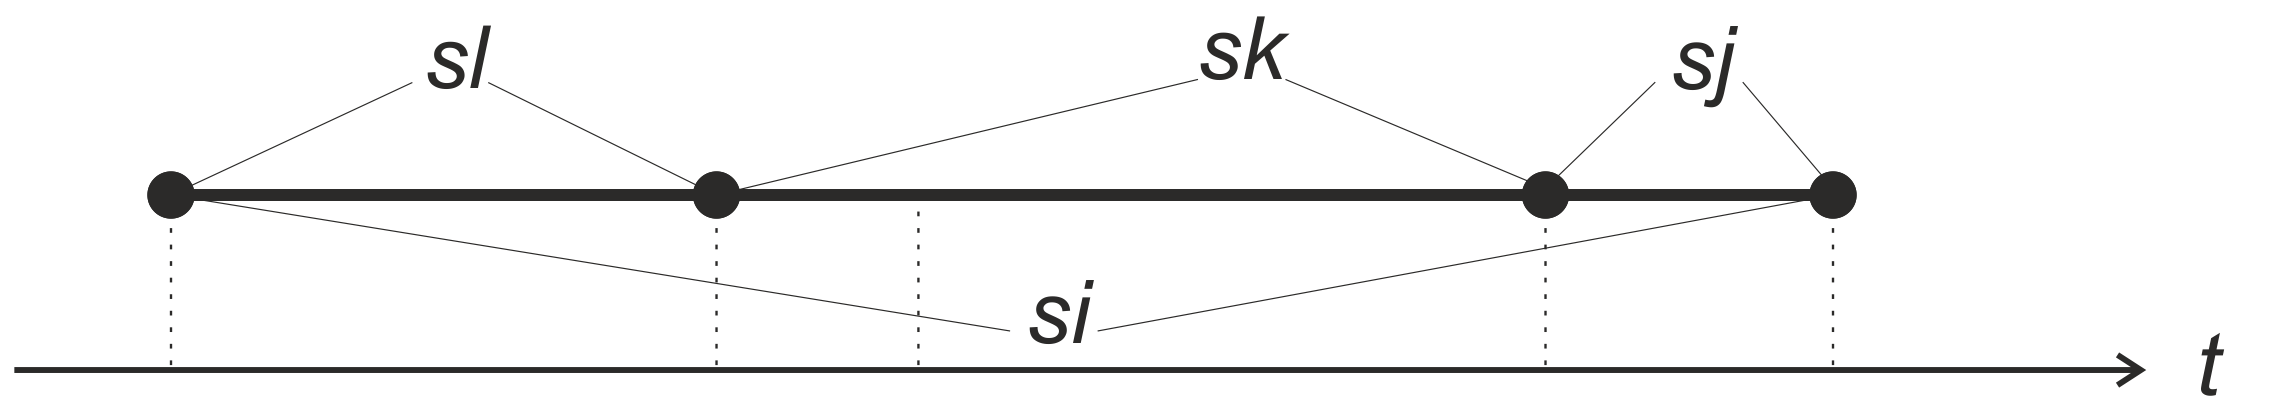
\includegraphics[width=\linewidth,height=0.68\textheight,keepaspectratio]{figures/sd_temp_entities/img_temporal_decomposition.png}
		\end{figure}
	\end{SCn}
\end{frame}

\begin{frame}{\\Temporal union}
	\topline
	\justifying
	\vspace{10mm}
	\begin{SCn}
		\begin{figure}[H]
			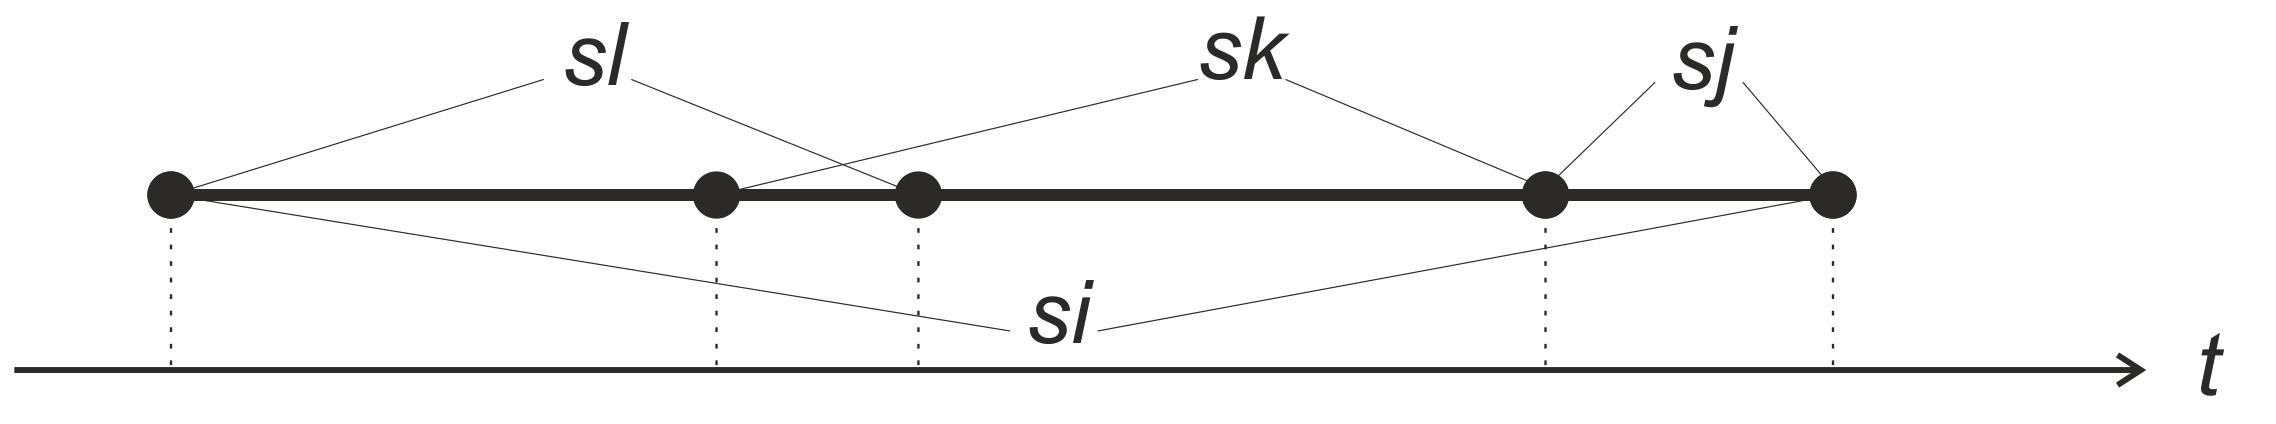
\includegraphics[width=\linewidth,height=0.68\textheight,keepaspectratio]{figures/sd_temp_entities/img_temporal_union.png}
		\end{figure}
	\end{SCn}
\end{frame}

\begin{frame}{\\Temporal union}
	\topline
	\justifying
	\vspace{10mm}
	\begin{SCn}
		\begin{figure}[H]
			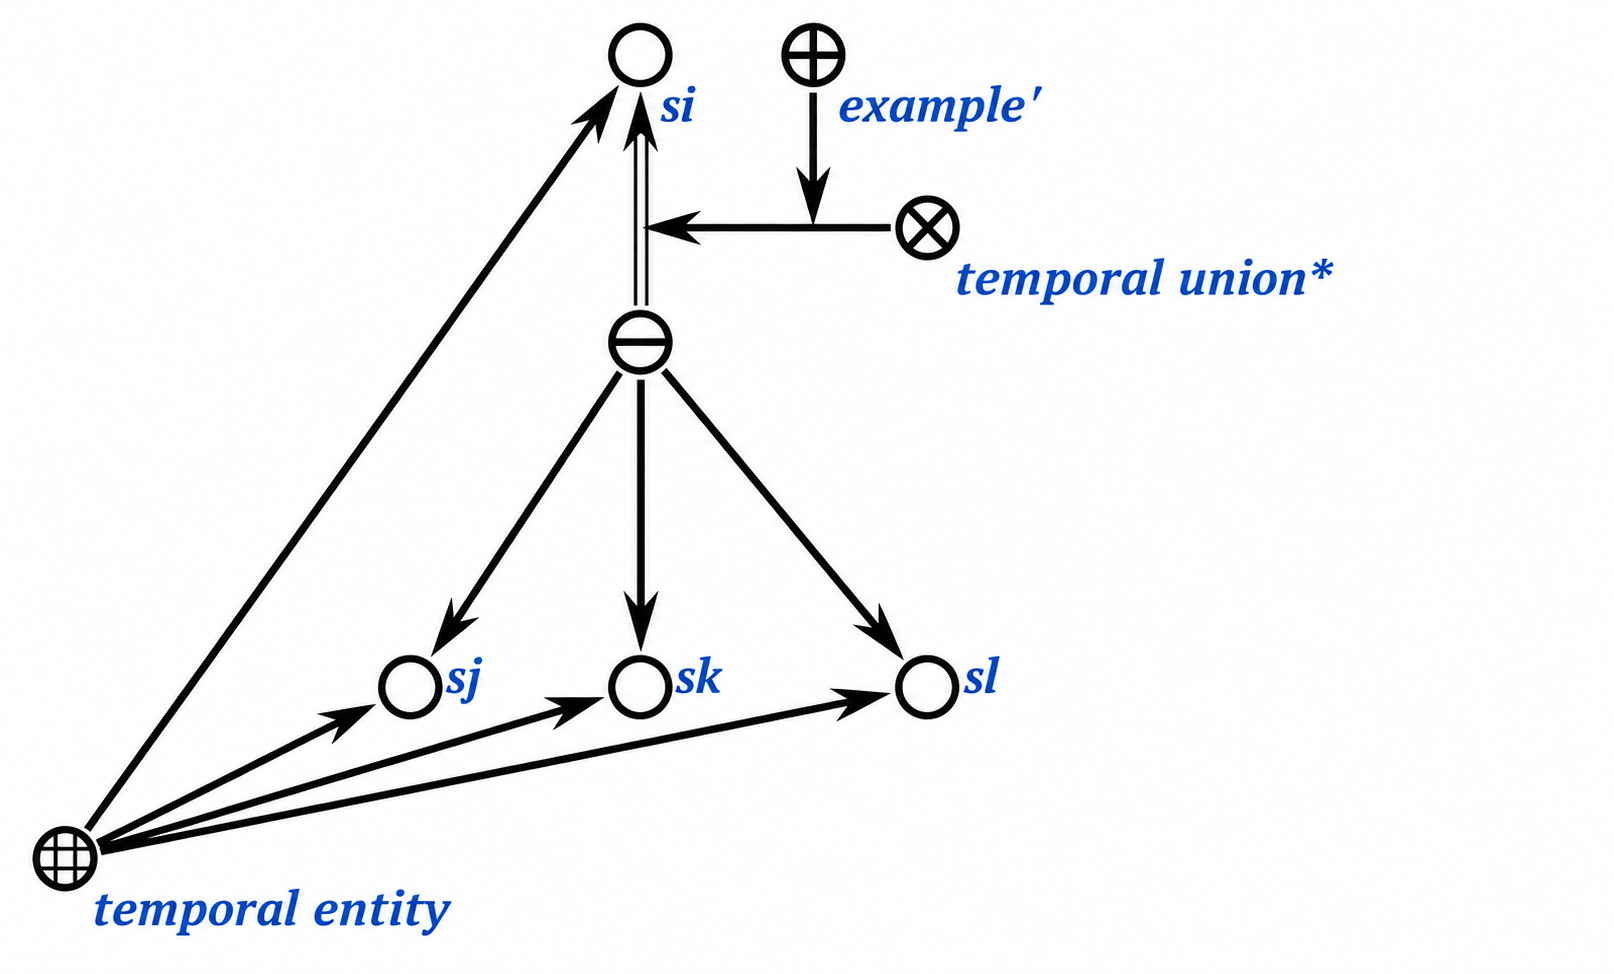
\includegraphics[width=\linewidth,height=0.68\textheight,keepaspectratio]{figures/sd_temp_entities/temporal_union_en.png}
		\end{figure}
	\end{SCn}
\end{frame}

\begin{frame}{Temporal inclusion}
	\topline
	\justifying
	\vspace{10mm}
	\scnheader{temporal inclusion*}
	\scntext{explanation}{Tuples of the \textit{temporal inclusion*} relation connect two temporal entities, one of whose periods of existence is entirely contained in the other's. The first component of each tuple is the sign of the longer-lived temporal entity.}
	\scnsuperset{temporal part*}
	\scnsuperset{temporal inclusion with distinct start and end times*}
	\scnsuperset{temporal coincidence*}
	\scnsuperset{temporal inclusion with coinciding start times*}
	\scnsuperset{temporal inclusion with coinciding end times*}
\end{frame}

\begin{frame}{\\Temporal parts, inclusion, and coincidence}
	\topline
	\justifying
	Tuples of the \textbf{temporal part*} relation connect two temporal entities, one of which is part of the other, such as an action and one of its subactions. The period of existence of one is therefore always contained in that of the other (the larger entity).\\
	The \textbf{temporal inclusion*} relation is more general: its tuples can connect any temporal entities.
	\scnheader{temporal coincidence*}
	\scnidtf{coincidence of start and end times*}
\end{frame}

\begin{frame}{\\Temporal part}
	\topline
	\justifying
	\vspace{10mm}
	\begin{SCn}
		\begin{figure}[H]
			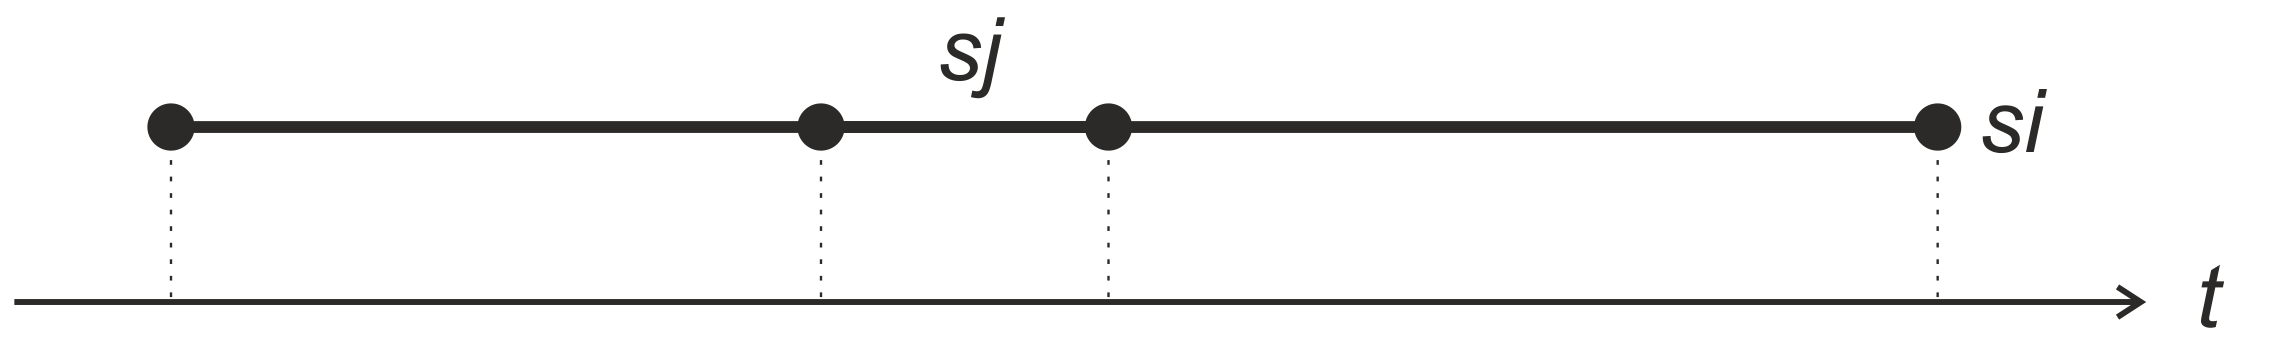
\includegraphics[width=\linewidth,height=0.68\textheight,keepaspectratio]{figures/sd_temp_entities/img_temporal_part.png}
		\end{figure}
	\end{SCn}
\end{frame}

\begin{frame}{\\Temporal inclusion (strict)}
	\topline
	\justifying
	\vspace{10mm}
	\begin{SCn}
		\begin{figure}[H]
			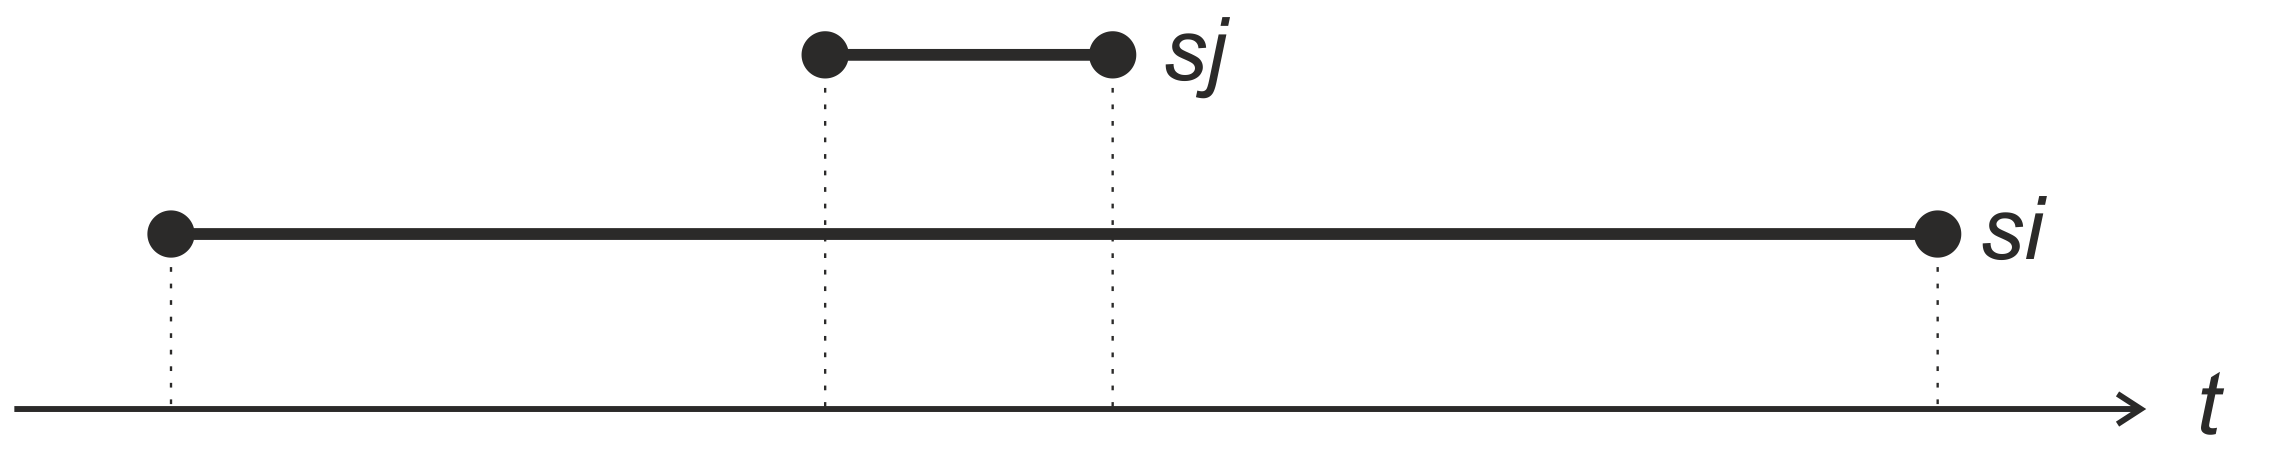
\includegraphics[width=\linewidth,height=0.68\textheight,keepaspectratio]{figures/sd_temp_entities/img_strict_temporal_inclusion.png}
		\end{figure}
	\end{SCn}
\end{frame}

\begin{frame}{Temporal inclusion (same start time)}
	\topline
	\justifying
	\vspace{10mm}
	\begin{SCn}
		\begin{figure}[H]
			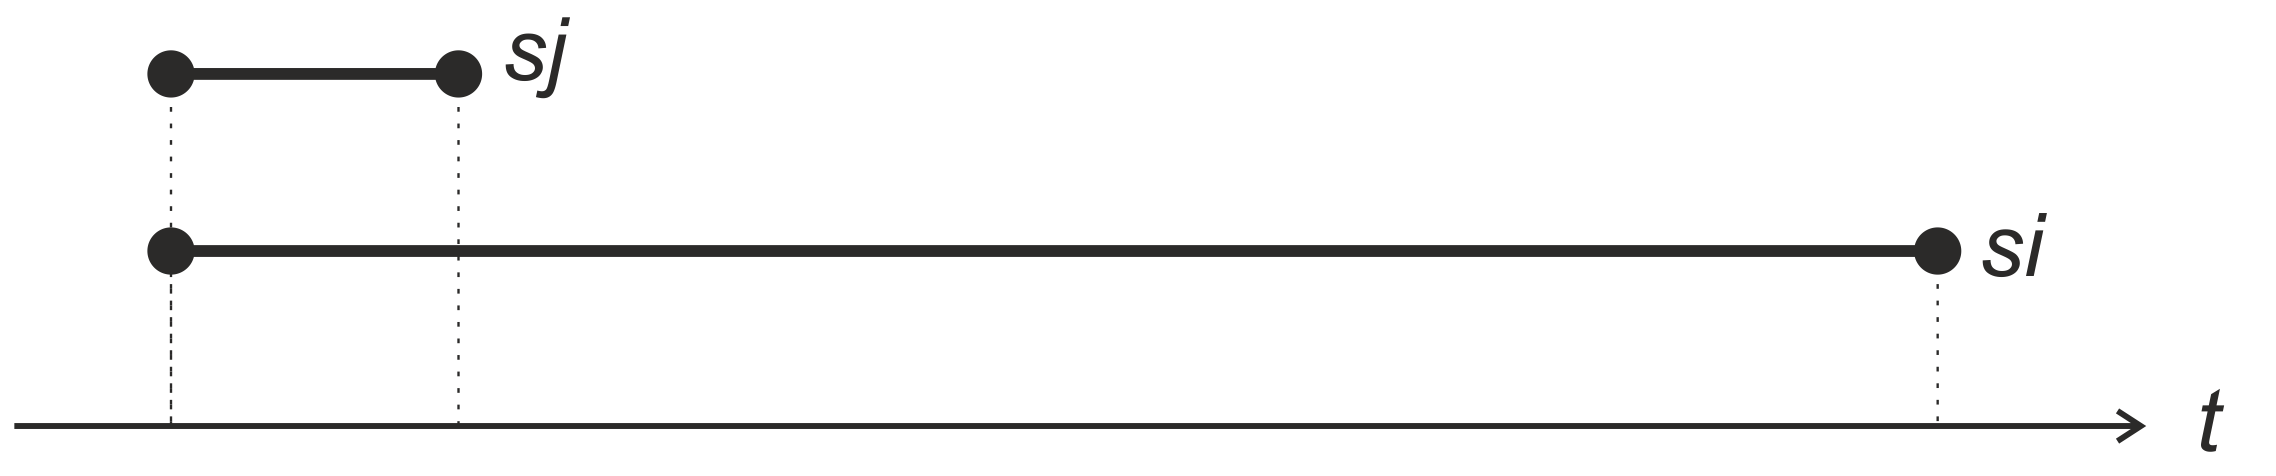
\includegraphics[width=\linewidth,height=0.68\textheight,keepaspectratio]{figures/sd_temp_entities/img_temporal_include_with_match_start_points.png}
		\end{figure}
	\end{SCn}
\end{frame}

\begin{frame}{Temporal inclusion (same end time)}
	\topline
	\justifying
	\vspace{10mm}
	\begin{SCn}
		\begin{figure}[H]
			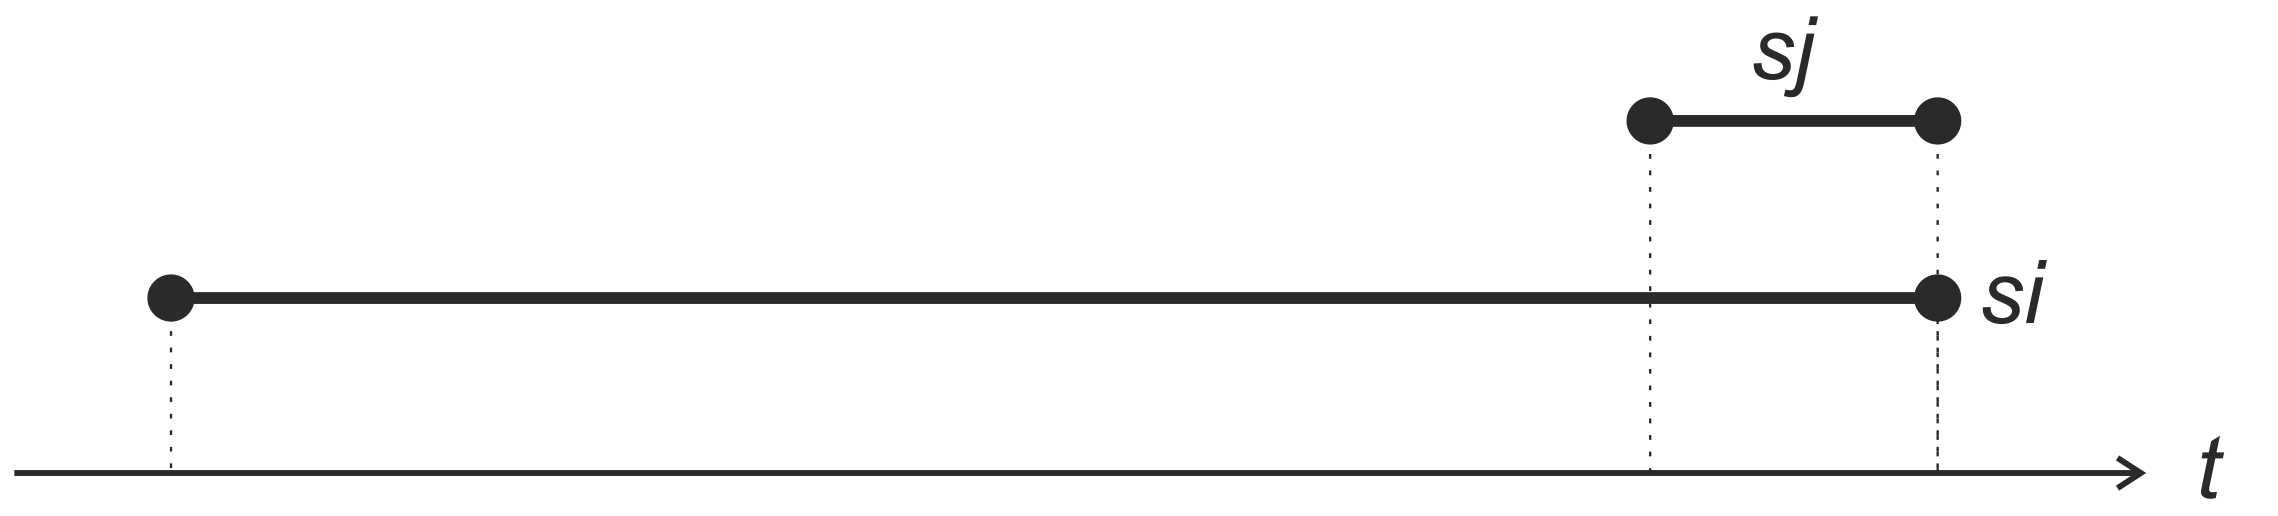
\includegraphics[width=\linewidth,height=0.68\textheight,keepaspectratio]{figures/sd_temp_entities/img_temporal_include_with_terminal_point_match.png}
		\end{figure}
	\end{SCn}
\end{frame}

\begin{frame}{\\Temporal adjacency}
	\topline
	\justifying
	\scnheader{temporal adjacency*}
	\scnidtf{temporal sequence with no gap*}
	\scnidtf{immediately after*}
	\scnheader{temporal sequence with overlap*}
	\scnheader{temporal sequence with a gap*}
	\scnidtf{not immediately after*}
\end{frame}

\begin{frame}{\\Temporal adjacency}
	\topline
	\justifying
	\vspace{10mm}
	\begin{SCn}
		\begin{figure}[H]
			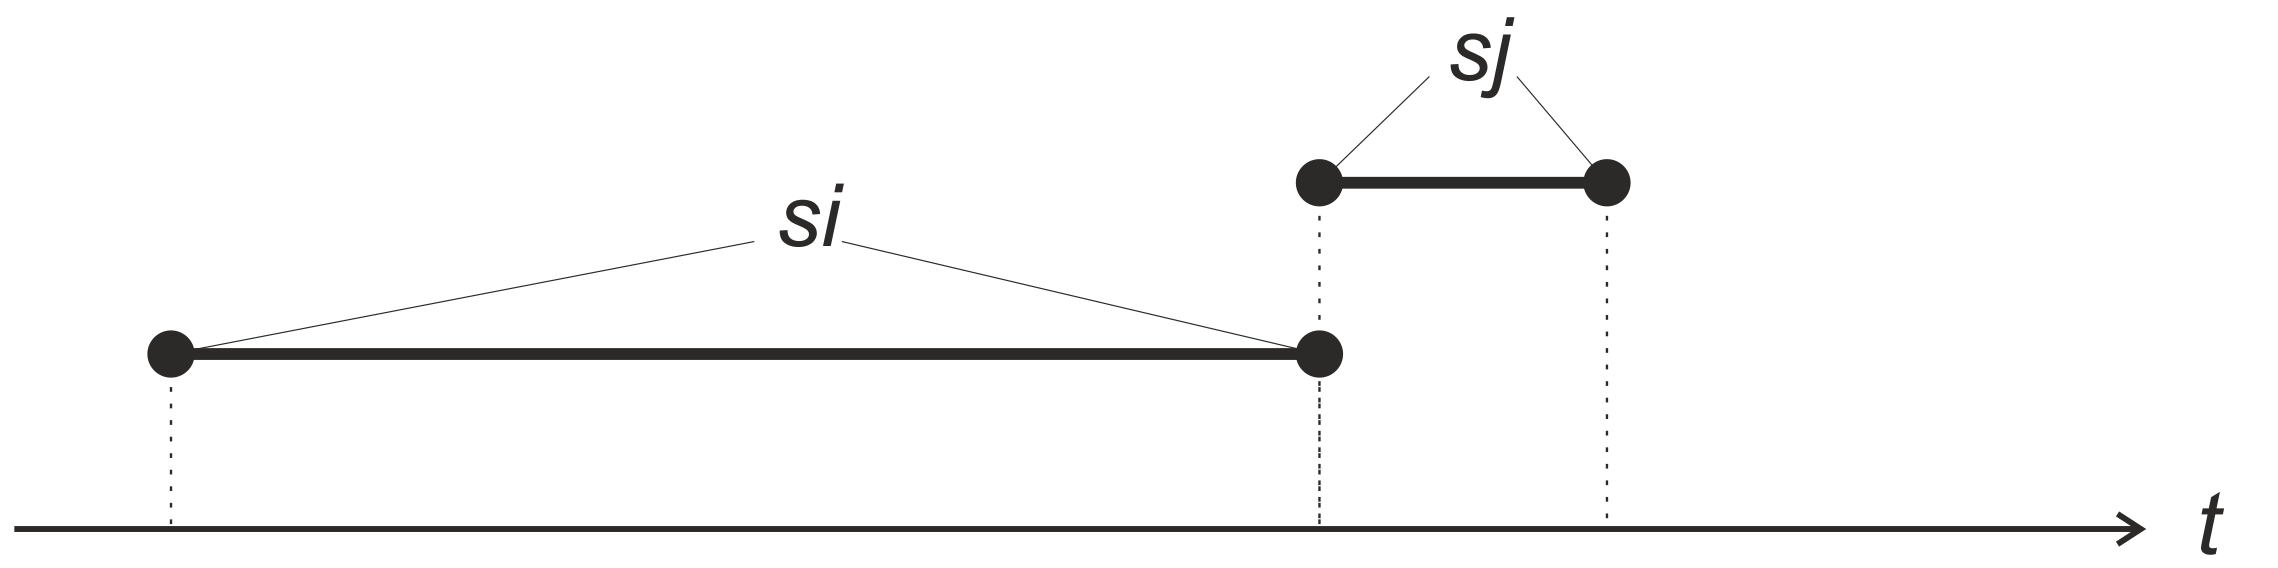
\includegraphics[width=\linewidth,height=0.68\textheight,keepaspectratio]{figures/sd_temp_entities/img_temporal_adjacency.png}
		\end{figure}
	\end{SCn}
\end{frame}

\begin{frame}{Temporal sequence with overlap}
	\topline
	\justifying
	\vspace{10mm}
	\begin{SCn}
		\begin{figure}[H]
			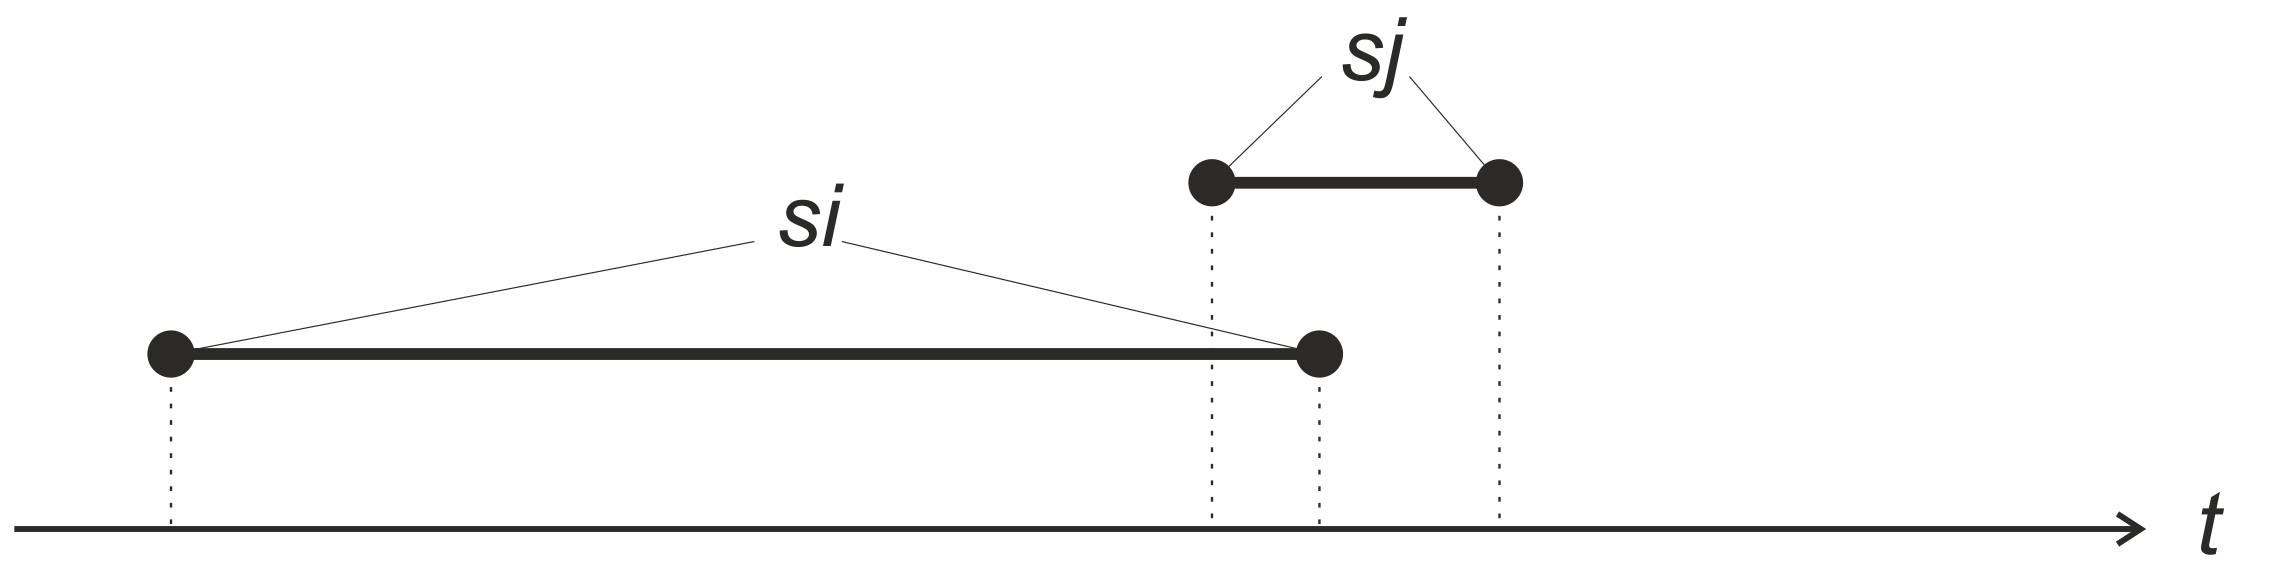
\includegraphics[width=\linewidth,height=0.68\textheight,keepaspectratio]{figures/sd_temp_entities/img_temporal_cross_sequence.png}
		\end{figure}
	\end{SCn}
\end{frame}

\begin{frame}{Temporal sequence with a gap}
	\topline
	\justifying
	\vspace{10mm}
	\begin{SCn}
		\begin{figure}[H]
			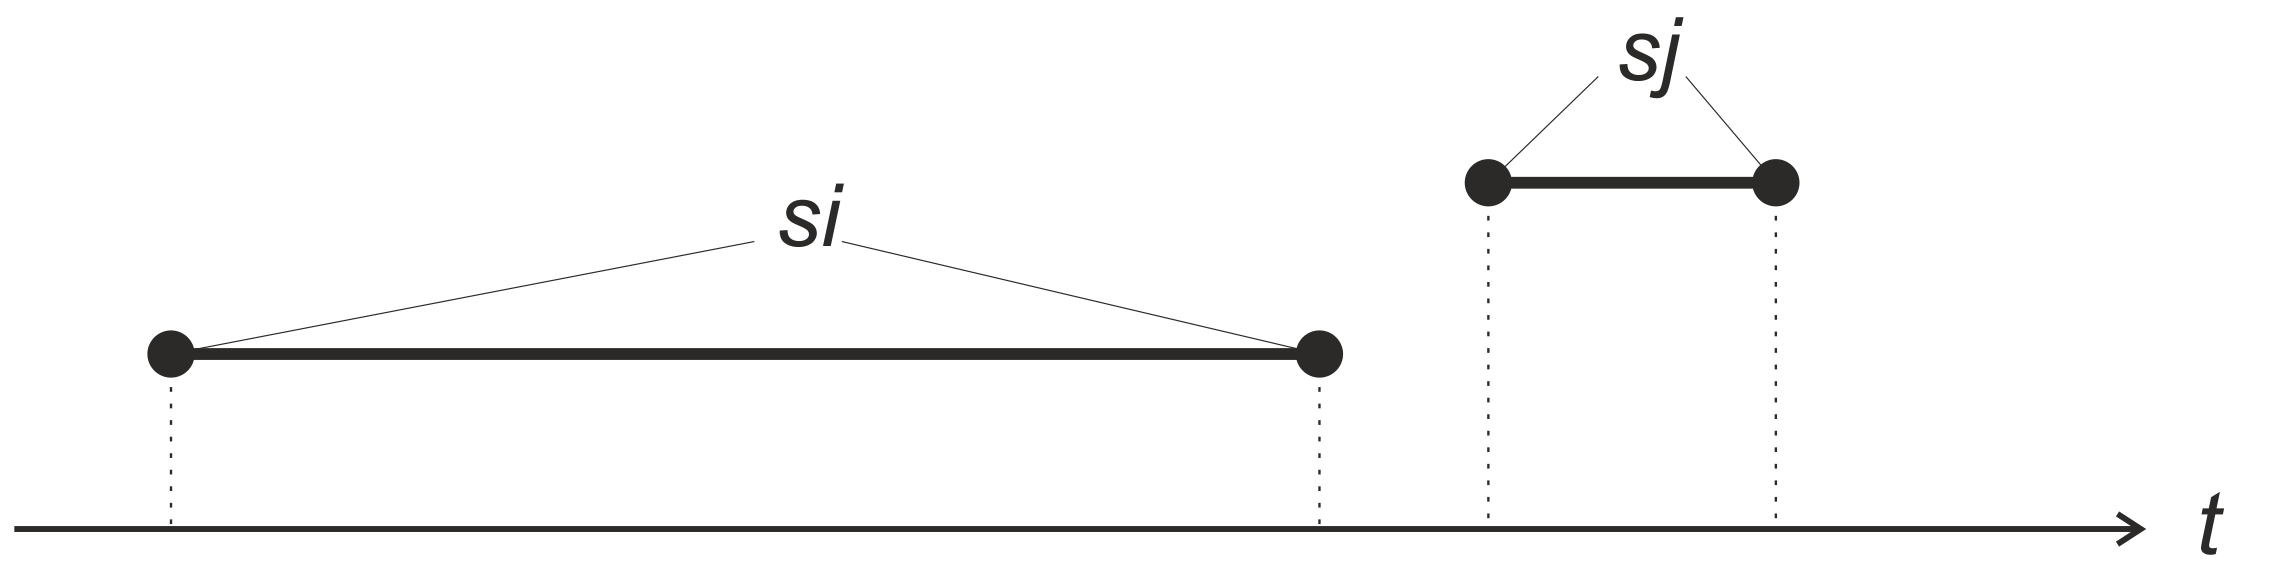
\includegraphics[width=\linewidth,height=0.68\textheight,keepaspectratio]{figures/sd_temp_entities/img_temporal_sequence_with_intermediate.png}
		\end{figure}
	\end{SCn}
\end{frame}

\begin{frame}{\\Temporal parameters}
	\topline
	\justifying
	\scnheader{parameter}
	\scnhaselement{duration}
	\scnhaselement{start}
	\scnhaselement{completion}
	\scnhaselement{simultaneity}
\end{frame}

\begin{frame}{\\Duration}
	\topline
	\justifying
	\vspace{10mm}
	\begin{SCn}
		\begin{figure}[H]
			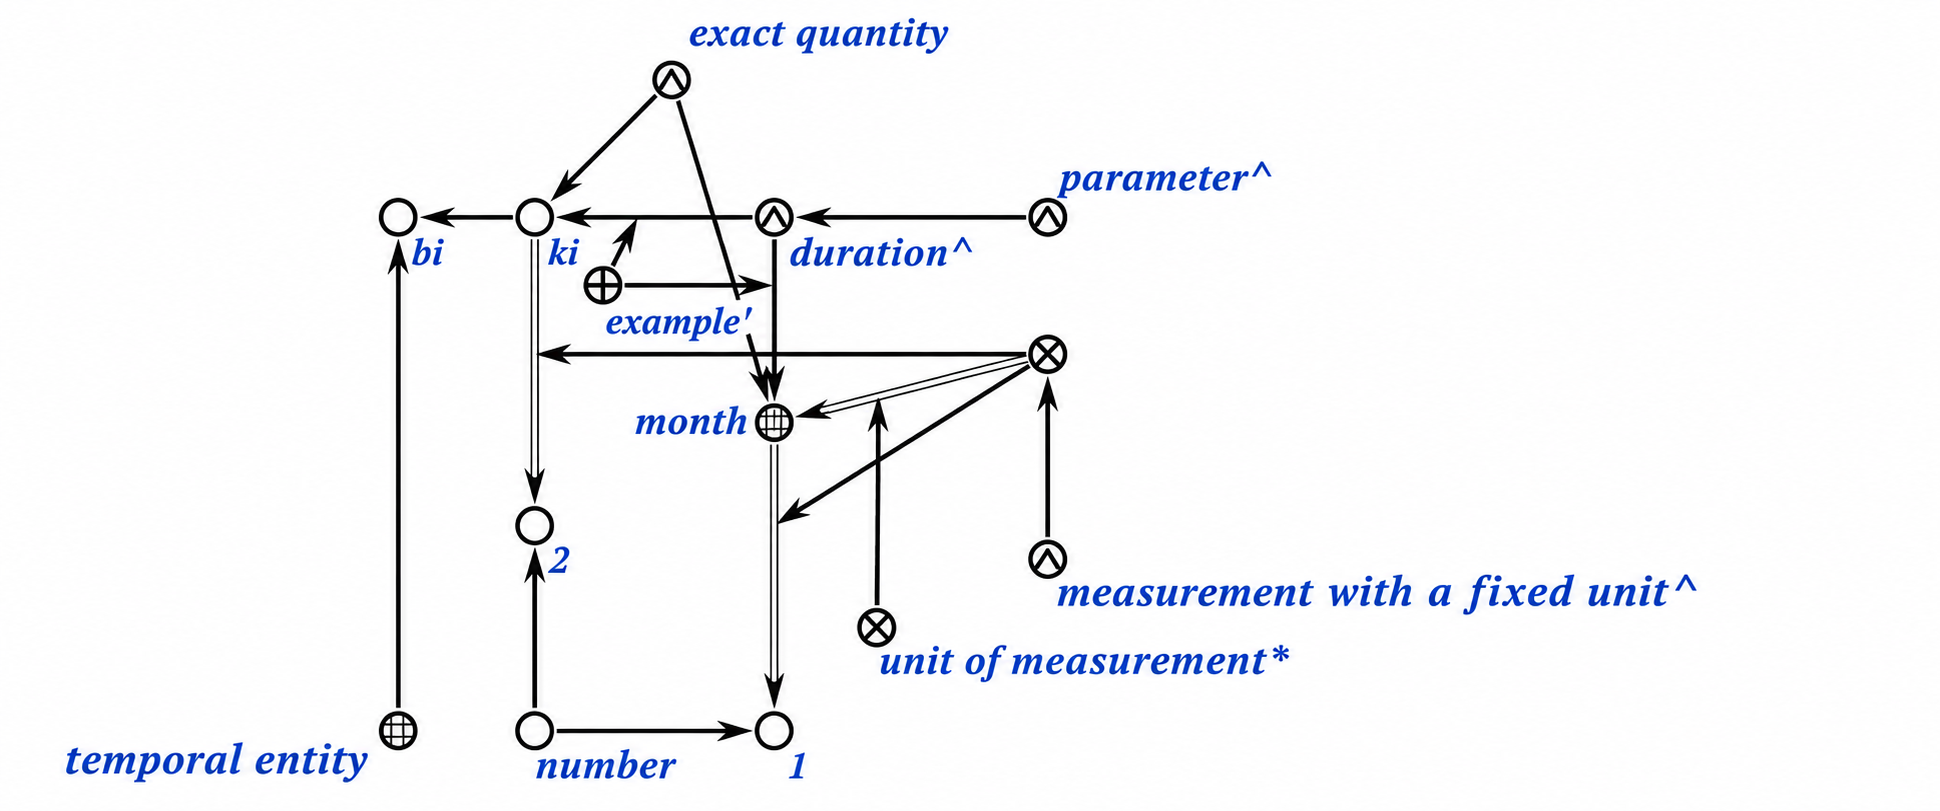
\includegraphics[width=\linewidth,height=0.68\textheight,keepaspectratio]{figures/sd_temp_entities/duration_en.png}
		\end{figure}
	\end{SCn}
\end{frame}

\begin{frame}{\\Completion}
	\topline
	\justifying
	\vspace{10mm}
	\begin{SCn}
		\begin{figure}[H]
			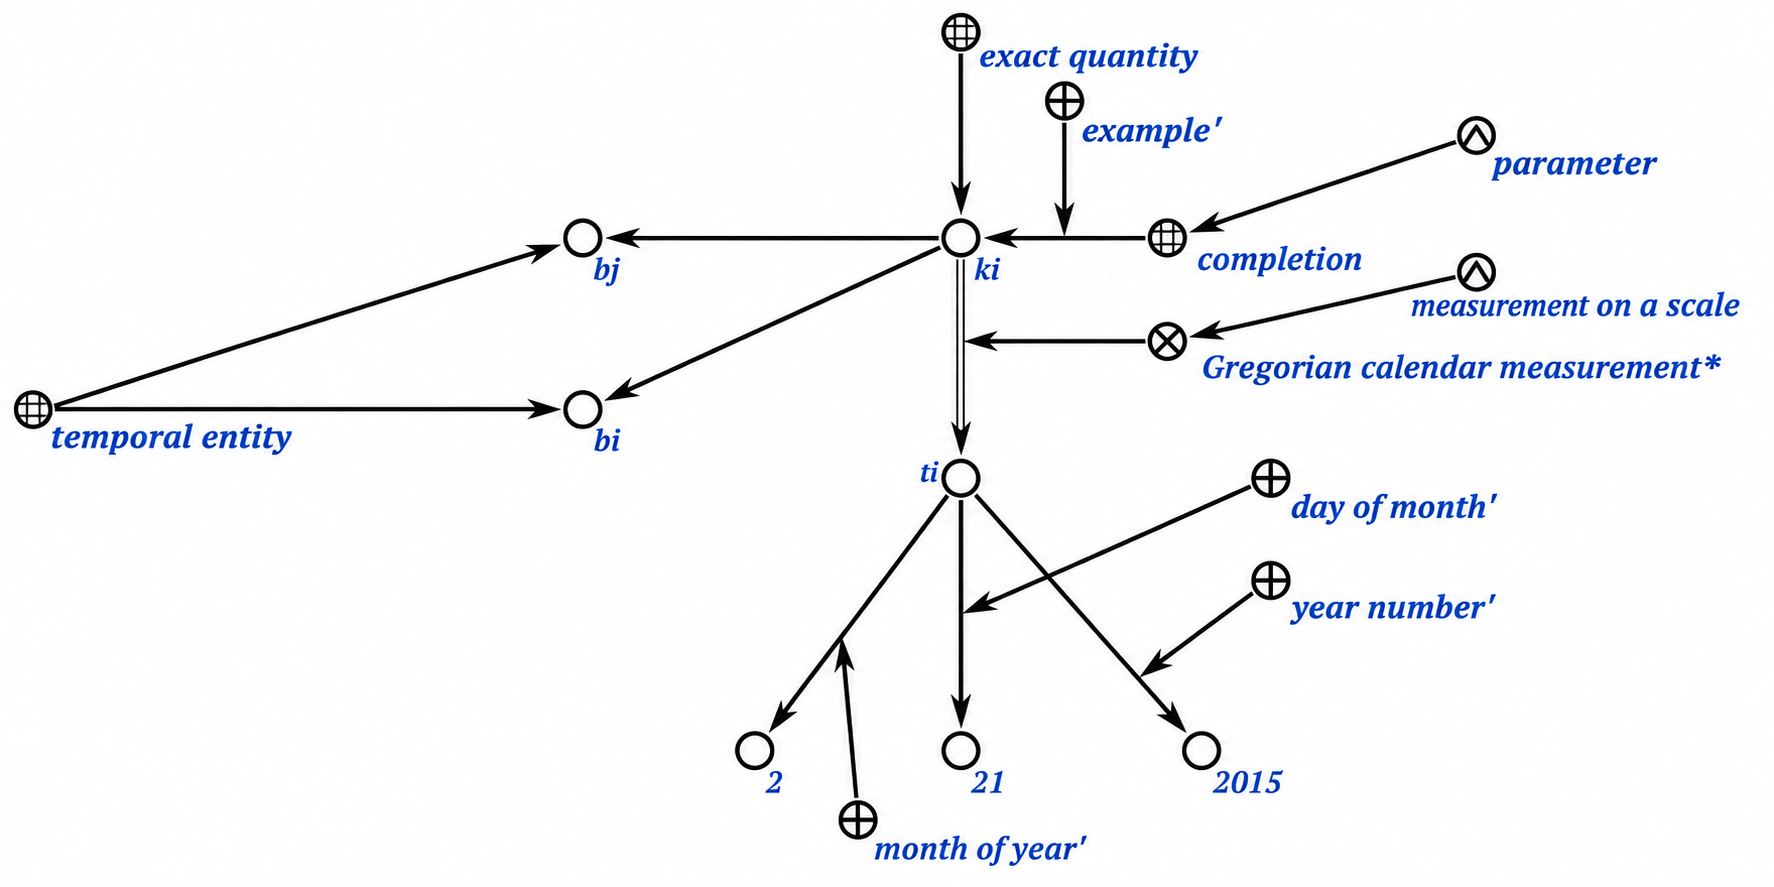
\includegraphics[width=\linewidth,height=0.68\textheight,keepaspectratio]{figures/sd_temp_entities/completion_en.png}
		\end{figure}
	\end{SCn}
\end{frame}

\begin{frame}{\\Simultaneity}
	\topline
	\justifying
	\vspace{10mm}
	\begin{SCn}
		\begin{figure}[H]
			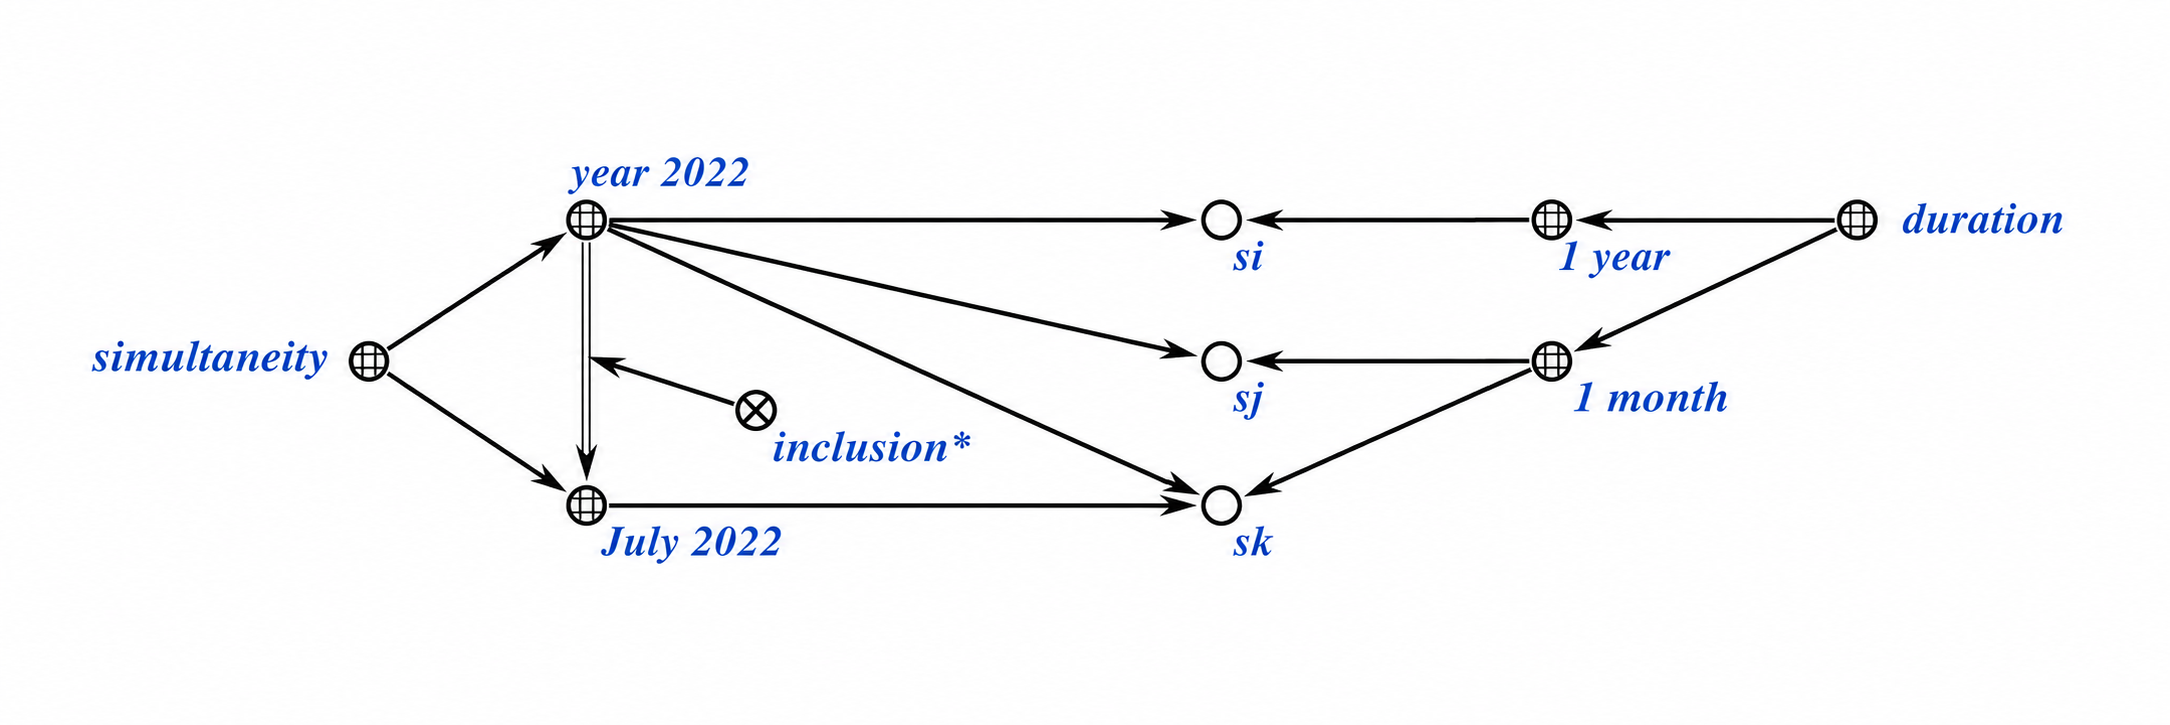
\includegraphics[width=\linewidth,height=0.68\textheight,keepaspectratio]{figures/sd_temp_entities/simultaneity_en.png}
		\end{figure}
	\end{SCn}
\end{frame}
